% Artifact mockup only. Not input by main.tex.
% Shows how Figure 10 would look if it replaced Table 17.
\documentclass[11pt]{article}
\usepackage[margin=1in]{geometry}
\usepackage[utf8]{inputenc}
\usepackage[T1]{fontenc}
\usepackage{mathptmx}
\usepackage{graphicx}
\usepackage{booktabs}
\usepackage{microtype}
\usepackage[font=small,labelfont=bf,labelsep=period]{caption}

\begin{document}
\pagestyle{empty}

\noindent\textit{Mockup page (not in the manuscript PDF). Table~17 remains in the paper.}

\vspace{1.2em}

\begin{figure}[h]
\centering
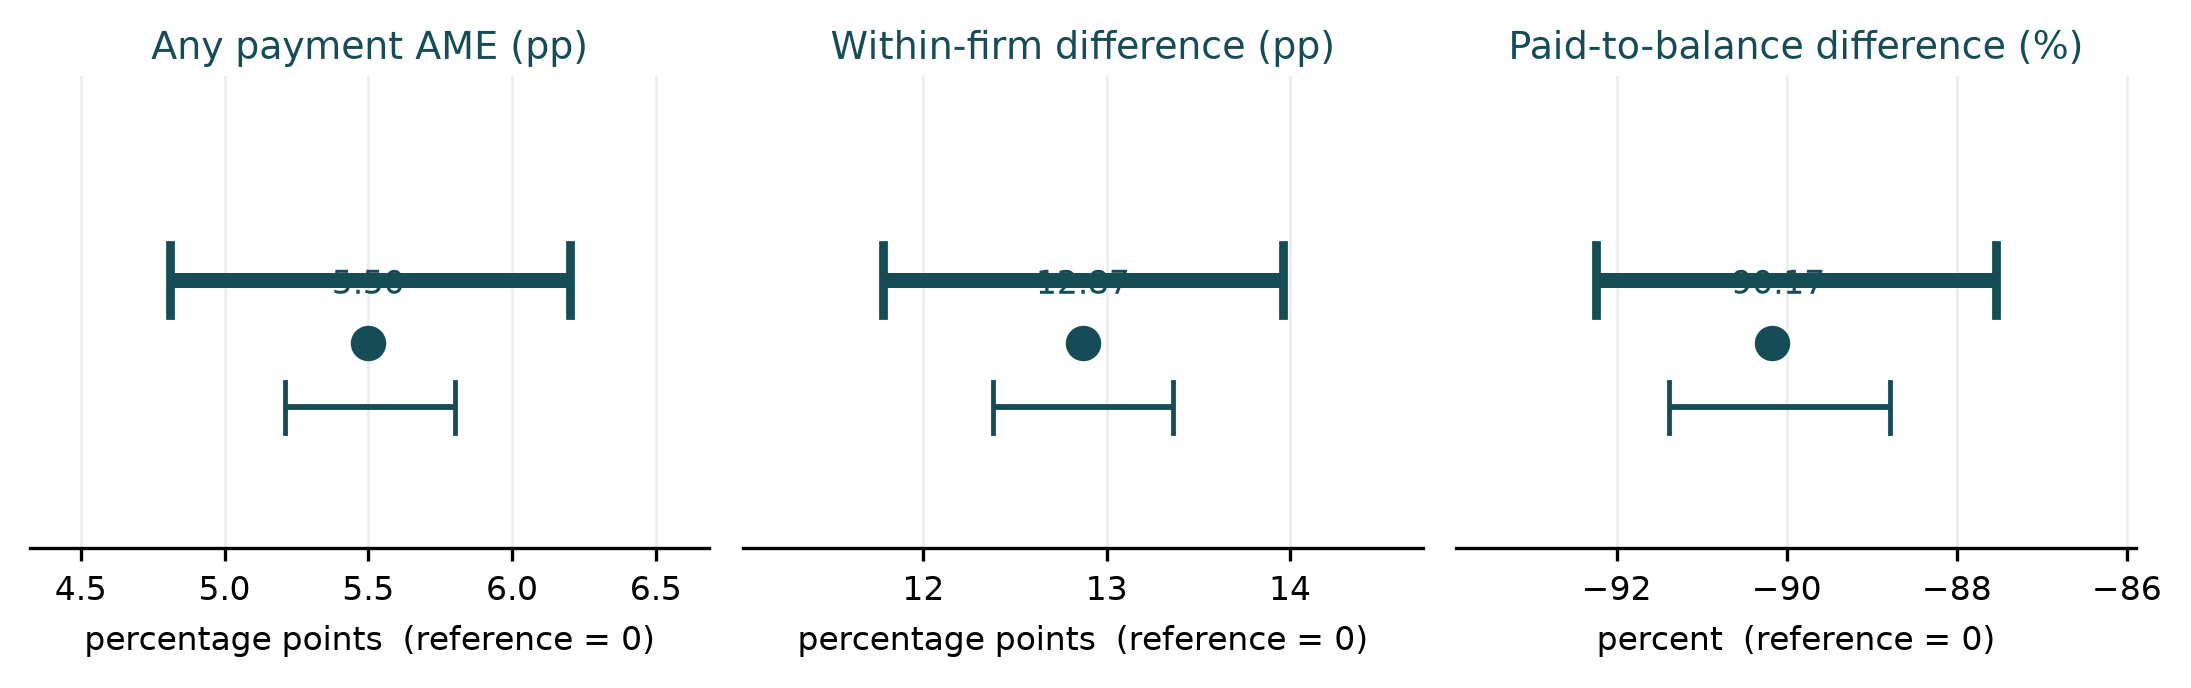
\includegraphics[width=\textwidth]{fig_origin_contrasts_v2.png}
\caption{Assessed origin relative to declared origin.
Each panel is one contrast from the committed model outputs.
The marker is the point estimate.
The thick bar is the cluster 95~percent interval.
The thin bar is the HC3 95~percent interval, drawn with a vertical offset so both intervals remain visible.
Each panel uses its own horizontal scale, zoomed to the estimate and intervals.
Where zero falls outside that scale, the axis label notes that the reference is zero.
The quantile regression of log stock is a separate equation.}
\end{figure}

\vspace{1.5em}
\noindent\footnotesize
Proposed caption above. Thick $=$ cluster (main). Thin $=$ HC3 (robustness). No legend box in the figure.
\end{document}
